

%Zur Dekodierung auf eine bestimmte Lautsprecheranordnung wird eine Matrix aus virtuellen Mikrofonen berechnet, woraus sich eine Tabelle mit Gain-Werten ergibt. Diese Tabelle besteht aus einer Spalte für jeden Lautsprecherkanal und kann die einzelnen Frequenzbins in einem VBAP-Verfahren den enstprechenden Lautsprechern zuordnen. In dieser Seminararbeit wurden dabei zwei Ansätze für die Dekodierung verglichen: Einerseits die direkte Dekodierung auf die physische Lautsprecheranordnung des Wiedergabesystems, und andererseits ein allgemeiner Ansatz womit die Dekodierung auf eine t-Design Lautsprecheranordnung erfolgt. Dieser Dekodierungsansatz hat den Vorteil, dass die Wiedergabeanordnung zum Zeitpunkt des Upmixings nicht vorgegeben sein muss. Auch für die Klangqualität ergeben sich daraus Vorteile, welche im Hörversuch besprochen werden.

Im Frequenzbereich wird jeder spektrale Block mit dem Sampling-Dekoder dekodiert, um die vier Eingangskanäle (B-Format) in eine höhere Kanalzahl zu wandeln.
In dieser Seminararbeit wurden dabei zwei Ansätze für die Dekodierung verglichen: Einerseits die direkte Dekodierung auf die physische Lautsprecheranordnung des Wiedergabesystems, und andererseits eine allgemeine Dekodierung auf ein t-Design. Dieser Dekodierungsansatz hat den Vorteil, dass die physische Lautsprecheranordnung zum Zeitpunkt des Upmixings nicht gegeben sein muss.

Bei einem 9-Design (Abb. \ref{fig:tdesign_image}) ergibt sich eine sphärische Anordnung von 48 virtuellen Lautsprechern, welche eine optimale Kodierung/Dekodierung des B-Formats vierter Ordnung erlaubt.

\begin{figure}[!ht]
  \centering
  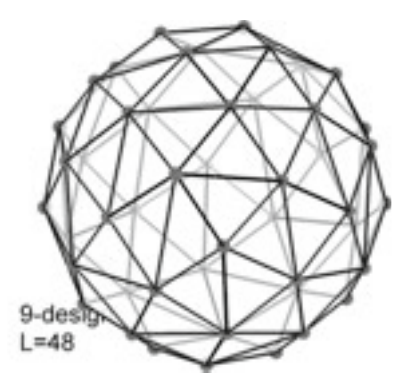
\includegraphics[width=0.35\textwidth]{implementierung/plots/t-design.png}
  \caption{9-Design T-Design \cite{ambi-book}}
  \label{fig:tdesign_image}
\end{figure}

%Zur Dekodierung wird in Octave also eine Matrix mit Lautsprechergewichten für Schalleinfallsrichtungen erstellt. Somit kann einer gegebenen frequenzabhängigen Richtung (bestehend aus Azimuth und Elevation), ein bestimmter Gain-Wert am entsprechenden Lautsprecherkanal zugeordnet werden.
